\documentclass[a4paper,12pt]{article}

\usepackage{tkz-euclide}
\usepackage{graphicx}
\usepackage{amsmath}

\begin{document}
\title{Assignment 4}
\author{Junaid Ahmad Bhat}
\date{16 January 2021}
\maketitle
\section*{\small Question}

$\triangle  ABC$ is right angled at B. If a = 12 and b+c =
18, find b, c and draw the triangle.

\section*{\small Solution}

Given \hspace*{3.8cm} a=12,\\

\vspace*{1mm}

and  \hspace*{3cm}  b+c=18;\\

$\Rightarrow$  \hspace*{3.5cm} c=18-b    \hspace*{1.5cm}(1)\\

Therefore,\\
\hspace*{0.5cm} we have 3 sides of given right triangle as BC=12,AC=b,AB=18-b.\\

By Pythagoras theorem,we have\\

\textbf{Hypotenuse$^2$=Base$^2$+Altitude$^2$}\\

As given triangle is right angled at B,side opposite to angle B is AC i,e b is\\

hypotenuse ,therfore,\\


 \hspace*{3cm} b$^2$=12$^2$+(18-b)$^2$\\ 

\vspace*{0.3cm}

 \hspace*{3cm} b$^2$=144+324+b$^2$-36b\\

\vspace*{0.3cm}

\hspace*{3cm} b=13 \hspace*{2cm}(2)\\

$\Rightarrow \hspace*{2.8cm} c=18-b \\
 \hspace*{4cm}=18-13 = 5$    \hspace*{1cm}(putting value of b from (2)in(1))\\



{\large So,the sides of triangle are:\textbf{ a=12,   b=13,  c=5}.}

\vspace*{1mm}

\subsection*{Steps of Construction:-}
 \hspace*{0.7cm }1.Draw a line AC of length =13(i,e b) .\\
	 
	 2.Taking A as centre draw an arc of radius =5(i,e c).\\
	 
	 3.Taking C as centre draw an arc of radius=12(i,e a).\\
	 
	 4.Name the point, where the two arcs meet(step 2 and step 3), as B.\\
	 
	 5.Join BA and BC.\\

      Required triangle is given below.\\
      
      Scale used:0.4*actual value.
      
      \vspace*{1cm}
          
\begin{center}
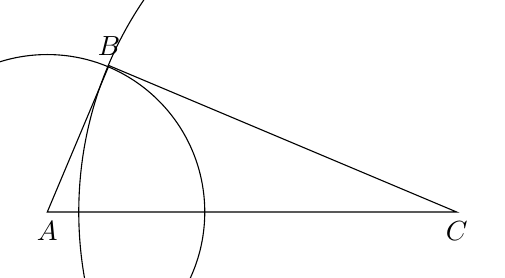
\begin{tikzpicture}

      \coordinate[label=below:$A$] (a) at (0,0);
       \coordinate[label=below:$C$] (b) at (5.2,0);
        \begin{pgfinterruptboundingbox}

        \node(Cric1) at (b) [draw,circle through=($ (b) + (0:4.8)$)]{};
         \node(Cric2) at (a) [draw,circle through=($ (a) + (0:2)$)]{};

\end{pgfinterruptboundingbox}
           \coordinate[label=above:$B$] (c) at (intersection 1 of Cric1 and Cric2);
\draw(b)--(a)--(c)--cycle;
\end{tikzpicture}
\end{center}

\pagebreak

\vspace*{5cm}


\begin{tikzpicture}
    	
		
       \coordinate [label=above:$A$] (A) at (0,5);
		\coordinate [label=left:$B$] (B) at (0,0);
		\coordinate [label=right:$C$] (C) at (12,0);
	
		\draw (B) -- node[left] {$\textrm{c(5)}$} (A) -- node[above]
		{$\textrm{b(13)}$} (C) -- node[below,,xshift=2mm] 
		{$\textrm{a(12)}$} (B);
		  
		\tkzMarkRightAngle[fill=black!10,size=0.8](A,B,C);
		  
\end{tikzpicture}
 
\hspace*{3cm} Figure of given triangle.

\vspace*{6cm}


%\textbf{* NOTE:we have used value of a=a/2.5,b=b/2.5 and c=c/2.5 in construction just to adjust the figure in the page,it would not effect the shape of triangle ,also the ratio of sides will remain same.}
 

\end{document}